\section*{Assignment 04: Monetisation Strategy}
\addcontentsline{toc}{section}{Assignment 04: Monetisation Strategy}

This section converts spreadsheet tests into a monetisation map while still in platform theory instead of wishful thinking.

\subsection*{Revenue options and theoretical grounding}
I listed four revenue streams and matched each principles from \citet{Choudary2016} and \citet{HagiuWright2013}.
\begin{itemize}
  \item \textbf{Completion fee.} A 7\% fee only triggers once both sides confirm delivery. Hagiu and Wright argue that transaction fees should align with realised value to avoid discouraging participation, so the fee stays invisible until success is logged.
  \item \textbf{Enablement subscription.} Larger partners can upgrade to a monthly enablement tier that bundles templated briefs, analytics, and advisory sessions. \citet{Choudary2016} lists producer tools as the second monetisation layer once the core interaction works, so this tier waits until the grow phase.
  \item \textbf{Insight reports.} Skill and impact trends can be sold to universities and municipal innovation teams. \citet{ShapiroVarian1999} note that information goods scale cheaply, yet \citet{Zuboff2019} warns about surveillance, so reports only launch with differential privacy, opt in consent, and the governance checks described in Assignment~05.
  \item \textbf{Grant funded scholarships.} Philanthropic grants and university funds can subsidise stipends for resource constrained NGOs. This follows \citet{ShapiroVarian1999}'s price discrimination guidance and keeps inclusion aligned with Assignment~07's fairness commitments.
\end{itemize}

\subsection*{Sequencing across the lifecycle}
I map timing to the seed, grow, scale arc from \citet{Choudary2016}.
\begin{enumerate}
  \item \textbf{Months 0 to 6.} No fees. The focus is on trust rituals: weekly office hours, onboarding, and a public map. Success means 30 completed projects and satisfaction above four point five.
  \item \textbf{Months 7 to 12.} Introduce the 7\% completion fee for new organisations while \textit{grandfathering} the founding cohort for three months (No fees). Pilot the enablement tier with five agencies and track completion above 85\%, churn below 10\%, and net promoter score above plus thirty. These thresholds come from lecture case studies on balancing monetisation with quality \citep{Lecture05}.
  \item \textbf{Month 12.} Extend fees to all partners, roll out enablement broadly, and launch the insight reports once the data board signs off on privacy safeguards. Monitor revenue per active organisation with engagement to catch risks in extraction \citep{Srnicek2017}.
\end{enumerate}

\subsection*{Experiments and cost discipline}
Each revenue stream is tested through paired tests. The completion fee runs an A/B test comparing when disclosure happens either at brief creation or after matching. The enablement tier uses \textit{Van Westendorp pricing interviews} with at least 20 organisations, and only launches if the acceptable range falls between 400 and 500 DKK. Insight reports begin with a diary study of 15 participants who rate trust on a five-point scale; scores below 3 trigger a redesign. Fixed year-one costs are about 620,000 DKK for product, design, and operations, while variable costs depend on finished sprints. Break-even requires roughly 1,050 projects a year, based on Assignment 09’s capacity model.

Figure~\ref{fig:student-profile} shows the student profile interface that makes these revenue streams plausible. It surfaces badges, skill evidence, and mentor quotes that organisations value, while prompts encourage students to keep data fresh. The mock up acts on \citet{Choudary2016}'s advice to monetise after creating tangible producer surplus.

\begin{figure}[H]
  \centering
  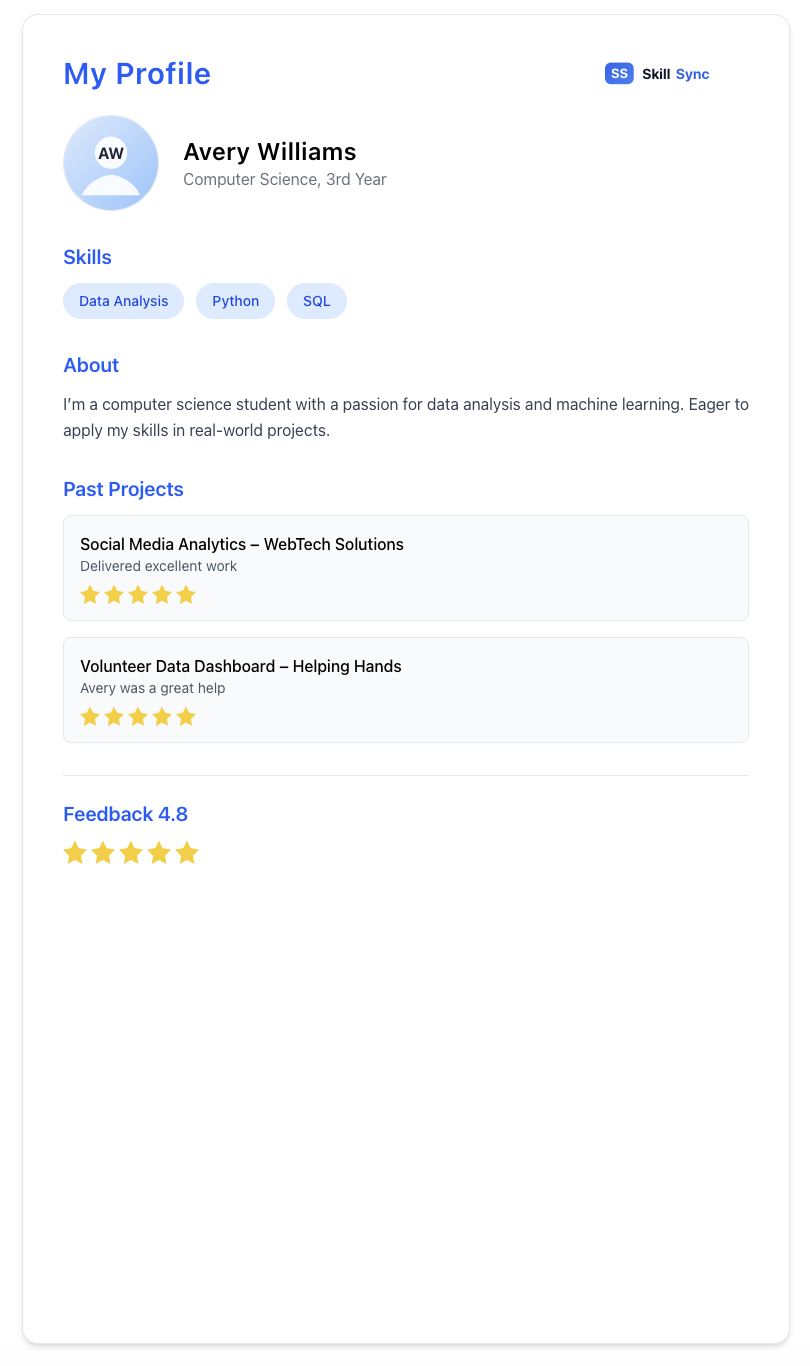
\includegraphics[width=0.8\linewidth]{figures/Student-Profile.png}
  \caption{Student profile mock up highlighting evidence that underpins monetisation.}
  \label{fig:student-profile}
\end{figure}

Ethical rules close the plan. Reports only start once at least five organisations in a sector and five hundred finished projects exist. Consent screens explain why each datapoint is collected, and grants stay separate from transaction fees to avoid bias. These measures turn \citet{Zuboff2019}’s critique into concrete product requirements.